\begin{figure}
  \centering
  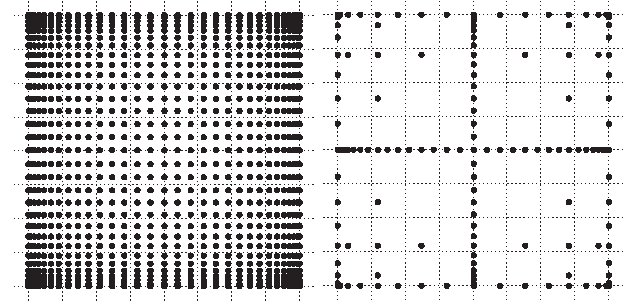
\includegraphics[width=0.9\linewidth]{include/assets/integration-grids.pdf}
  \vspace{-1.0em}
  \caption{A full-tensor product grid (on the left) and a Smolyak sparse grid (on the right) \cite{eldred2008}.}
  \flabel{integration-grids}
  \vspace{-1.0em}
\end{figure}

As mentioned in \sref{polynomial-chaos}, \sref{ie-polynomial-chaos}, and \aref{polynomial-chaos}, the coefficients of PC expansions are integrals, which should be calculated numerically at \stage{4}.
In numerical integration, an integral of a function is approximated by a summation over the function values computed at a set of prescribed points, or nodes, which are multiplied by the corresponding set of prescribed weights.
Such pairs of nodes and weights are called quadrature rules \cite{press2007}.
A one-dimensional quadrature rule is characterized by its precision $\qdprecision$, which is defined as the maximal total order \cite{heiss2008} of polynomials that the rule integrates exactly.
In multiple dimensions, an $\nvars$-variate quadrature rule is formed by tensoring one-dimensional counterparts. Such a multidimensional rule is characterized by the level of accuracy $\qdlevel$, which is defined as the index of the rule in the corresponding family of multidimensional rules with increasing precision.

It can be seen in \eref{inner-product} that the integrand can be decomposed into two parts: the weight function, $\fPDF(\vz)$, and everything else.
The former stays the same for all inner products; therefore, an integration rule is typically chosen in such a way that the corresponding weights take into consideration this ``constant'' part since there is no point of recomputing $\fPDF(\vz)$ each time when the other part, \ie, the functions that the inner product operates on, changes.
Consequently, there exist different families of quadrature rules tailored for different weight functions.
Define such a quadrature-based approximation of the inner product in \eref{inner-product} as follows:
\[
  \oInner{h(\vz)}{g(\vz)} \approx \oQuad{\nvars}{\qdlevel}{h(\vz) \: g(\vz)} := \sum_{i = 1}^{\qdorder} h(\qdn{\vz}_i) \: g(\qdn{\vz}_i) \: \qdw_i
\]
where $\qdn{\vz}_i \in \real^\nvars$ and $\qdw_i \in \real$ are the prescribed nodes and weights, respectively; $\qdorder$ is their number; and $\qdlevel$ is the accuracy level of the quadrature rule, which is said to be $\nvars$-variate.
Note that, once the rule to use is identified, $\qdn{\vz}_i$ and $\qdw_i$ are fixed, \ie, there is no any additional computational effort.
In our experiments in \sref{experimental-results}, we use the library of quadrature rules available at \cite{burkardt2013}.

Since in the example in \sref{illustrative-example} we need to compute inner products with respect to beta measures, the Gauss-Jacobi quadrature rule is of particular interest.
The rule belongs to a broad class of rules known as Gaussian quadratures, which implies that its order $\qdorder$ and precision $\qdprecision$ are related as $\qdprecision = 2 \qdorder - 1$; this feature makes such quadratures especially efficient \cite{heiss2008}.
Consequently, we rewrite \eref{pc-coefficients} as follows:
\[
  \pcc{\vP}_{ki} = \frac{1}{\pcn_i} \oQuad{\nvars}{\qdlevel}{\vP_k(\o) \pcb_i(\vZ(\o))}
\]
where $\{ \pcn_i \}_{i = 1}^{\pcterms}$ are computed exactly, either by directly using the same quadrature rule or by taking products of the one-dimensional counterparts with known analytical expressions \cite{xiu2010}; the result is further tabulated.
It is important to note that $\qdlevel$ should be chosen in such a way that the rule is exact for polynomials of the total order at least $2 \pcorder$, \ie, twice the order of the PC expansion, which can be seen in \eref{pc-coefficients} \cite{eldred2008}.
Therefore, $\qdlevel \geq \pcorder + 1$ as the quadrature is Gaussian.

There is one more and, arguably, the most crucial aspect of numerical integration that we ought to discuss: the algorithm used to construct multidimensional quadratures.
In low dimensions, the construction can be easily based on the direct tensor product of one-dimensional rules.
However, in high dimensions, the situation changes dramatically as the number of points produced by this approach can easily explode.
For instance \cite{heiss2008}, if a one-dimensional rule has only four nodes, \ie, $\qdorder = 4$, then in 10 dimensions, \ie, $\nvars = 10$, the number of nodes becomes $\qdorder^\nvars = 4^{10} = 1,048,576$, which is not affordable.
Moreover, it can be shown that most of the points obtained in such a way do not contribute to the asymptotic accuracy and, therefore, are a waste of time.
In order to effectively alleviate this problem, we construct so-called sparse grids using the Smolyak algorithm \cite{eldred2008, burkardt2013, heiss2008}.
The algorithm preserves the accuracy of the underlying one-dimensional rules for complete polynomials while significantly reducing the number of integration nodes.
For instance, in the example given earlier, the number of nodes computed by the algorithm would be only $1,581$.
In order to give a better appreciation of Smolyak's technique, \fref{integration-grids} displays an example \cite{eldred2008} where a full-tensor product grid is plotted side by side with a sparse grid of the same integration power.\footnote{This example uses a Clenshaw-Curtis quadrature rule, which is an important alternative to Gaussian quadratures; see \cite{eldred2008} for further details.}
Each dot in the figure is an evaluation of the function being integrated.
It can be seen that the Smolyak algorithm allows for drastic savings of the computational time.
